
\subsection{Caching layers}
\label{sec:cache-design}

%In the following, we present our \sysname~\preconstructcachename design.
%Each \texttt{pull layer} request has a precedent \texttt{pull manifest} request.
%Upon receiving a \texttt{pull manifest} request, 
%\sysname~sends the updated \sysname~manifest to client.
%After receiving a \sysname~manifest, the client parses the manifest
%and sends either a \texttt{pull layer} request if the layer hasn't been deduplicated,
%or a list of \texttt{pull slice} requests if a list of corresponding slices presents in the manifest.
%Those \texttt{pull slice} requests will then be
%forwarded to all the registry servers that store the requested
%layer's slices as shown in Figure~\ref{fig:sys-overview}. 

%\begin{figure}[t]
	\centering
	\centering
	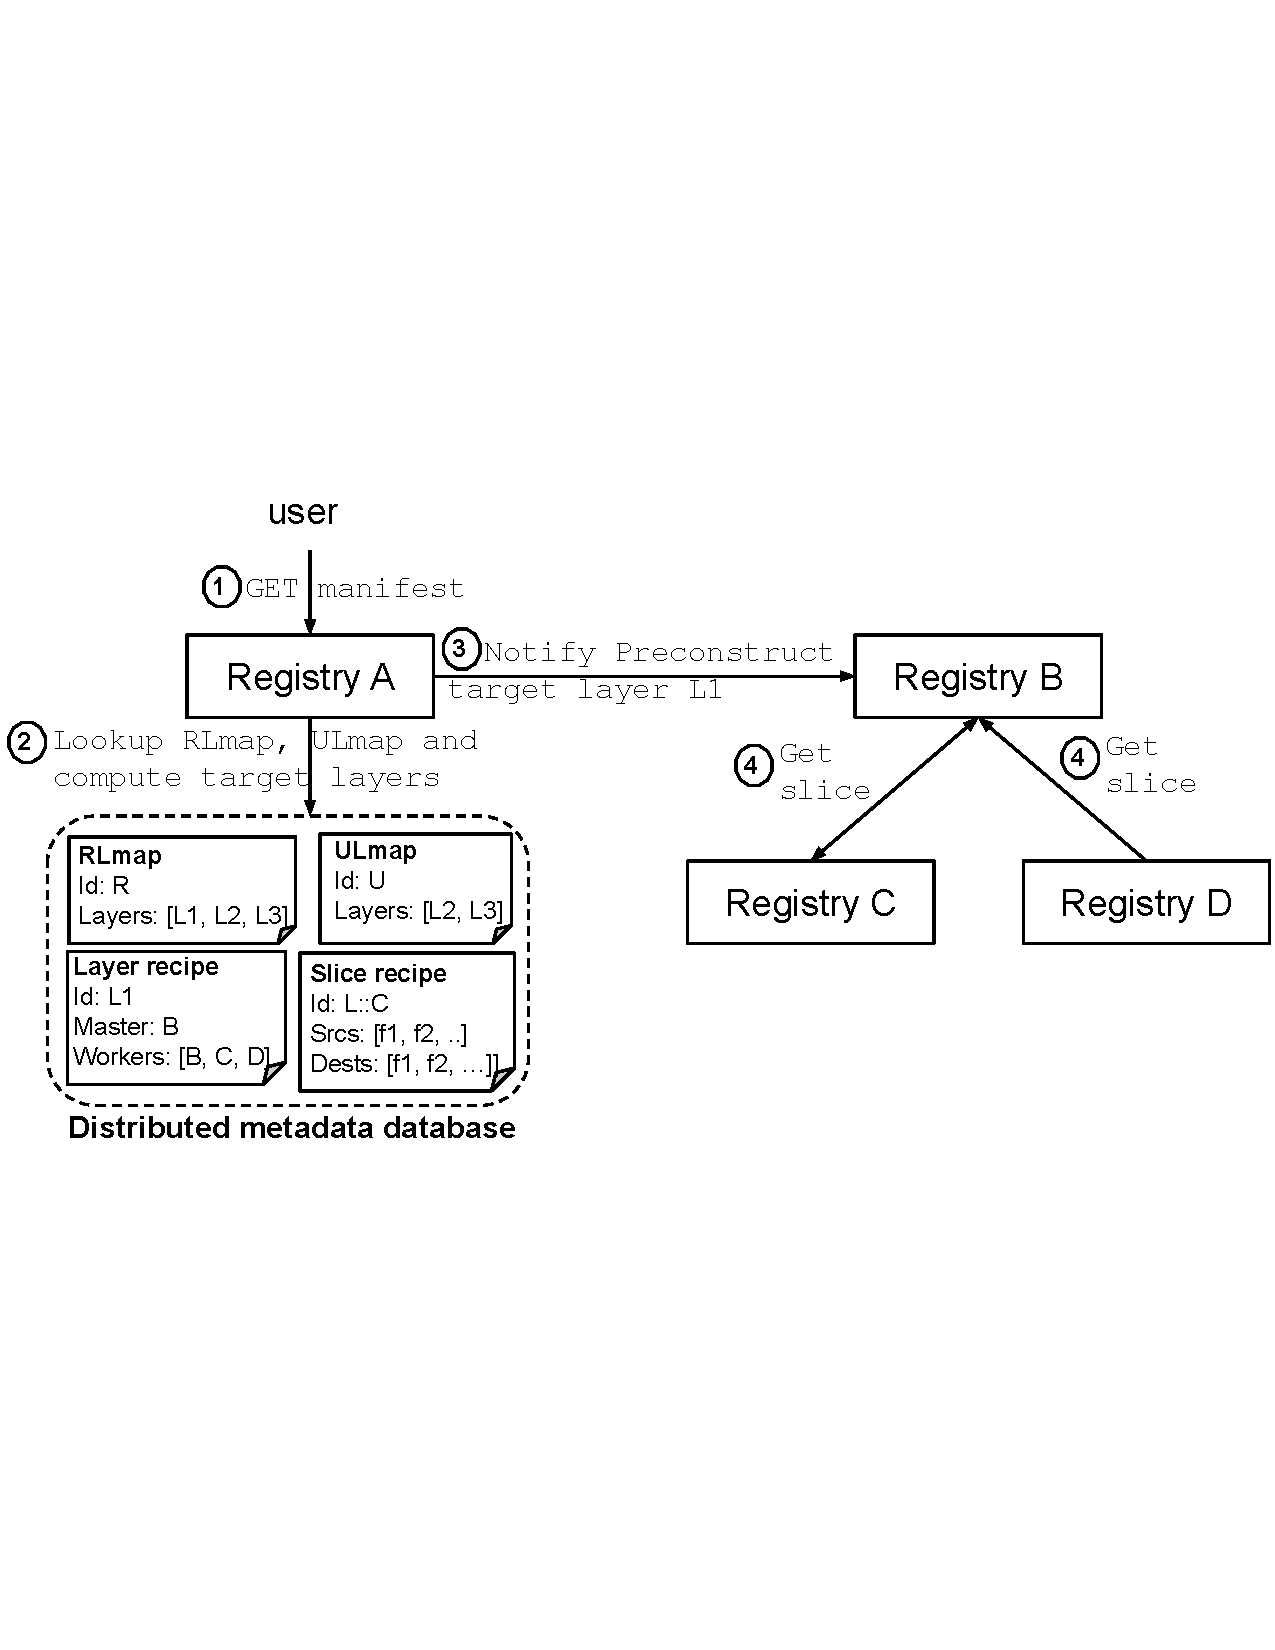
\includegraphics[width=0.49\textwidth]{graphs/sift-preconstruct.pdf}
	\caption{Layer preconstruction.}
	\label{fig:preconstruct}
\end{figure}

%\LR{Why are we calling it `superfetch cache'? Isn't that just a prefetch cache?}

\sysname maintains a cache layer in both the primary and deduplication clusters to speed up
\texttt{pull} requests. The primary cluster cache (also called \emph{superfetch cache}) is
memory-based to avoid disk I/O during layer retrievals while the deduplication cluster cache
(also called \emph{preconstruct cache}) is on disk. The main purpose of the preconstruct
cache is to store preconstructed layers, which are likely to be accessed in the future,
to avoid the layer restoring overhead.

Both caches are filled based on the user access patterns observed in Section~\ref{sec:dataset-analysis}.
\LR{Describe the interaction between the caches. Are they independent and make their
own predictions. Are they always making the same predictions? How large are they?}
\NZ{Yes, they have the same prediction module to do layer prediction and 
	share the metadata ULmap and RLmap.
But the two cache wont do prediction at the same time.
Either of them can do prediction and update the maps.}
%
%\sysname predicts what layers will be accessed and 
%prepares the layers before \texttt{pull} layer requests.
%To improve the performance of primary cluster,
%\sysname \emph{superfetches} the layers that will be accessed later into \textbf{superfetch cache}.
%Moreover,  to improve the layer restoring performance of deduplication cluster,
%\sysname preconstructs layers before \texttt{pull} layer requests 
%and put them into \textbf{preconstruct cache} to save restoring latency.

\paragraph{Request prediction}
%
%\LR{The following paragraph should be part of the background. By now,
%the reader should be familiar with the pull process.}
%
%Typically, when a user 
% \texttt{pulls} an image,
%it will first \texttt{pulls} the image's manifest and extract the image's layers from the manifest, 
%Next, it compares these layers against a \emph{local layer index}.
%If a layer isn't presents in the \emph{local layer index}, meaning the layer hasn't been stored locally,
%the user will \texttt{pull} the layer.
%Otherwise, the user will start pulling the layer.

%Based on the above access pattern,
To accurately predict layers that will be accessed in the future, \sysname keeps
track of user access patterns and image metadata.
Therefor, it uses two maps to record the image-to-layer information
and user layer accesses: RLmap and ULmap.
%
\LR{What do the abbrevations RL and UL stand for?}
\NZ{Repo to layers; User to Layers.}
%
\LR{ Is the layer set the set of layers contained in an image? Why do we need
an extra map for this? Can we also get this from the manifest? Need to explain
the reasoning here.}
\NZ{It takes a long time to load manifest for each request.}

RLmap maps an image to its containing \emph{layer set} and an entry in RLmap
is identified as \textless{}Repository name@manifest digest\textgreater.
%
%Layer is identified as layer digest.
%
ULmap stores for each user, the layers the has user accessed and the corresponding pull count.
A user is uniquely identified by extracting the sender network address from the request.

When a \texttt{GET manifest} request $r$ is received,
\sysname first calculates a set of image layers that haven't been pulled by the user $r.addr$ 
by calculating the difference $S_{\Delta}$ between the image's layer set and the user's accessed layer set
%
\begin{equation*}
S_{\Delta} = RLmap[r.img] - ULmap[r.addr].
\end{equation*}
%
The resulting layers in $S_{\Delta}$ are likely going to be accessed later.

Recall from \S\ref{sec:predictable-user-access} that some users \emph{always} pull
layers, no matter if the layers have been previously pulled. To detect such users,
\sysname first gets the subset, $S_{\cap}$, of layers from the image that have already
been pulled by the user by computing
%
\begin{equation*}
S_{\cap} = RLmap[r.img] \cap ULmap[r.addr].
\end{equation*}
%
Next,  \sysname compares the client repull probability 
$\gamma[r.addr]$ with a predefined client repull threshold $\varepsilon$.
If $\gamma[r.addr] > \varepsilon$, then \sysname classifies the user as a repull user
and fetches the layers in $S_{\cap}$ into the cache.
%
\LR{Here, we need to talk more about how we get the repull probability and how we
maintain it over time. Do we assume a static one like dicussed in background or
are we updating it for each client over time?}
\NZ{We calculate the repull proabability as the total number of pull layer request divided by the number of
it accessed layers.
We maintain each layer's pull count for a user in ULmap.
So we can calculate the repull probability during each prediction.}
%
%targets $\leftarrow$ difference \\
%\ForEach{layer in intersection} 
%{ \If{ layer.rpcnt $>$ $\theta_{rpc}$}{
%		targets	$\leftarrow$ layer
%	}
%}

\paragraph{Cache handling in tiered storage} 
%As mentioned earlier, \sysname uses two-tier storage architecture: primary cluster
%and deduplication cluster. Now with the adding of superfetch cache and preconstruct
%cache, The two-tier storage architecture becomes multiple-level storage architecture
%as shown in Figure~\ref{fig:tieredstore}.

\LR{We need to provide more details on how we search the different tiers.
Do we keep an index for each tier? How fast are the searches?}
\NZ{Layer index holds the server address for each layer replica.
	If the server is a P-server, then it's a layer replica stored in tier 1.
	Otherwise it is deduplicated and stored in tier  2.
Similar as files, we dont maintain layer path because each layer is stored in directory
‘rootdir/docker/registry/v2/blobs/sha256/< first two hex bytes of layer digest >/<hex layer digest>/’ 
(denoted as layerdir) as a file named ‘data’.
}

The introduction of the two cache layers results in a 5-tier storage architecture of
\sysname as shown in Figure~\ref{fig:tieredstore}. Requests are passed through the
tiers in the order displayed in the figure. Upon a \texttt{GET} layer request,
\sysname first searches the superfetch caches in primary cluster.
If the layer is present the request will be served from cache.
Otherwise, the request will be served from the layer store in the primary cluster.
%\texttt{prefetches} layers on primary cluster based on the above user request prediction theory.
%After P-servers receive the primary layer replicas,
%\sysname will save the layer replicas into \emph{superfetch cache} as shown in Figure~\ref{fig:sift}.
%Meanwhile, it updates \emph{RLmap} with the layer and its associated image. 

If a \texttt{GET} layer request can't be served from the primary cluster
due to a failure of the corresponding P-server(s),
the request will be forward to the deduplication cluster.
\sysname will first search the layer stage areas on the D-servers to check,
whether the requested layer has been recently uploaded.
If not found, \sysname will search the preconstruct caches and
finally, if not found, it will rebuild a layer to serve the request.

Both the superfetch and the preconstruct cache are write-through caches.
When a layers is evicted, it will simply be discard since it does not contain any
updates to layers. Recently uploaded layers, which are temporarily stored in the
layer stage area will be evicted to the preconstruct cache after the layer is
deduplicated.
%
\LR{Add details on eviction policies for each cache.}
We use Adaptive Replacement Cache (ARC) replacement~\cite{xxx}, 
which keeps track of both frequently used and recently used layers
and adapts to changing access patterns.
%For preconstruct cache, it's possible when a \texttt{pull} layer request comes 
%before layer restoring is finished, meaning the layer cannot be preconstructed \emph{on time}.
%In this case, \texttt{pull} layer request \emph{waits} until the restoring is finished
%(detailed in Section~\ref{sec:impl}).
%
%When a~\texttt{pull} layer request is received, 
%\sysname will first search superfetch cache for the request layer.
%If the layer presents in cache, the request will be served from cache.
%Otherwise,
%the request will be served from layer store.
%Meanwhile, it updates \emph{ULmap} with the request sender and its associated layer. 

%ULmap records user access status,
%which maps a \textbf{user Id} to its accessed layers with its corresponding access count,
%where user id is defined as client request address.

%
%\paragraph{Preconstruct cache on deduplication cluster}
%%\begin{algorithm}
\scriptsize 
	\caption{Layer preconstruction}
	\label{alg:prefetch}
	\KwIn{\\
		$\theta_{rpc}$: Threshold for repull layers to be preconstructed. \\
		$RLmap$: Repository to layer map. \\
		$ULmap$: User to layer map.  \\
		$LayerRecipes$: Layer recipes. \\
		$SliceRecipes$: Slice recipes.\\
	}
	\emph{r} $\leftarrow$ \texttt{request received}\\
	\uIf{r = GET manifest}
		{
			difference $\gets$ \emph{RLmap[r.repo]} $-$ \emph{ULmap[r.client]} \\
			intersection $\gets$ \emph{RLmap[r.repo]} $\bigcap$ \emph{ULmap[r.client]} \\
			
			targets $\leftarrow$ difference \\
			\ForEach{layer in intersection} 
			{ \If{ layer.rpcnt $>$ $\theta_{rpc}$}{
				targets	$\leftarrow$ layer
				}
			}
			\ForEach{layer in targets} {
				master $\leftarrow$ \emph{LayerRecipes[layer].master} \\
				\texttt{Notify} master `PRECONSTRUCT layer' \\
			}
		}
	
		\uElseIf{r = PRECONSTRUCT layer}
		{
			\If{r.layer not in DiskCache}{
				workers $\leftarrow$ \emph{LayerRecipes[r.layer].workers} \\
				\ForEach{worker in workers} {
					%{\scriptsize $/*$\textit{sliceid = r.layer+worker}}\\ 
					slices $\leftarrow$ \texttt{GET slice from} worker `GET slice' \\
				}
				layer $\leftarrow$ \texttt{Concatenate} slices \\
				
				DiskCache $\gets$ layer \\
				{\tiny{$/*$\texttt{Set timer for layer}} $/*$}\\
			}
		}
	
		\uElseIf{r = GET slice}
		{
			slice $\leftarrow$ \texttt{Construct by following} \emph{SliceRecipes[r.slice]} \\
			
			\texttt{Serve} slice \\
		}
	
%		\uElseIf{r = PUT layer}
%		{
%				\emph{LayerCache} $\leftarrow$ \texttt{cache} \emph{r.layer} \\
%				\texttt{update} \emph{RLmap[r.repo, r.layer]} \\
%		}
%		\uElseIf{r = GET layer} 
%		{
%			{\tiny\texttt{/* r.layer has not been deduplicated   /}} \\
%				\eIf{r.layer in cache}
%				{
%					\emph{cache hit for layer} \\
%					\texttt{Serve} layer \\
%				} 
%				{
%					workers $\leftarrow$ \emph{LayerRecipes[layer].workers} \\
%					\ForEach{slave in slaves} {
%						slices $\leftarrow$ \texttt{GET} worker `GET layer'slice' \\
%					}
%					layer $\leftarrow$ \texttt{Concatenate} slices \\
%					\texttt{Serve} layer
%					LayerCache $\gets$ layer \\
%				}
%		}
%		\texttt{update} \emph{ULmap[r.client, r.repo, r.layer]} \\
		
\end{algorithm}



%To improve layer restoring performance,
%\sysname \texttt{preconstructs} layers before \texttt{pull} layer requests to save layer construction time.
%Upon each \texttt{pull} manifest request,
%\sysname will predict a \emph{target layer set} that will be requested later based on above prediction theory.
%%
%%Meanwhile,
%%\sysname will update \emph{RLmap} with the layer and its associated repository, where
%%RLmap maps a \textbf{repository id} (i.e., repository name) to its containing layers 
%%as shown in Figure~\ref{fig:dedup-partition}.
%After that,
%\sysname gets each layer's layer recipe from metadata database
%and extracts each layer's restoring master.
%Next,
%\sysname sends a notification of \texttt{preconstruct layer} to
%each restoring master.
%After receiving the notification, 
%the restoring master starts layer restoring process and stores the preconstructed layer into \emph{preconstruct cache}.
%
%When a~\texttt{pull} layer request is received, 
%\sysname will first search requested layer from preconstruct cache.
%If the layer presents in cache, the request will be served from cache.
%Otherwise,
%\sysname will rebuild a layer from file store.


%(detailed in Section~\ref{xxx}).
 
%the request will be served from layer store.
%\sysname will first update \emph{ULmap}. 
%ULmap records user access status,
%which maps a \textbf{user Id} to its accessed layers with its corresponding access count,
%where user id is defined as client request address.

%Figure~\ref{fig:preconstruct}
%shows how to preconstruct layers for later accesses.
%When a \texttt{GET manifest} request is received by registry $A$,
%it gets the requested repository information and client information from RLmap and ULmap respectively, 
%and computes a list of target layers that will be accessed later by this client.
%As shown, to preconstruct target layer $L1$, 
%registry $A$ gets $L1$'s layer recipe from metadata database
%and sends a notification of \texttt{preconstruct layer} $L1$ to 
%$L1$'s restoring master: registry $B$. 
%After receiving the notification, 
%$B$ sends \texttt{get slice} requests to its peer workers: $C$ and $D$.
%When $B$, $C$, and $D$ finished slice constructions for $L$,
%three slices are concatenated by $B$ and saved in $B$'s layer diskcache. 


%
%Algorithm~\ref{alg:prefetch} shows how to determine target layers 
%based on observed user access pattern.
%When a \texttt{GET manifest} request \emph{r} is received,
%\sysname~gets a set of layers associated with the requested repository \emph{r.repo} from RLmap, 
%denoted as $RLmap[r.repo]$.
%Meanwhile, it also gets a set of layers associated with the client \emph{r.client} from ULmap,
%denoted as $ULmap[r.client]$.
%After that, it calculates a list of layers in the requested repository 
%that have not been \texttt{pulled} by the client by
%computing the difference set between $RLmap[r.repo]$ and $ULmap[r.client]$ (denoted as $difference$).
%All the layers in $difference$ are included in target set.
%\sysname also calculates a intersection set between 
%$RLmap[r.repo]$ and $ULmap[r.client]$ (denoted as $intersection$).
%The layers in $intersection$ are already pulled by client.
%To determine whether a layer in $intersection$ will be
%$repulled$ by client,
%\sysname compares its repull count against a predefined threshold $\theta_{rpc}$.
%If the layer's repull count is greater than $\theta_{rpc}$,
%which means this layer will be repulled with high probability.
%Thus, it is included in target layer set.

%After D-servers receive the backup replicas,
%\sysname will first update \emph{RLmap} with the layer and its associated repository, where
%RLmap maps a \textbf{repository id} (i.e., repository name) to its containing layers 
%as shown in Figure~\ref{fig:dedup-partition}.

%
%For each layer in target set, 
%\sysname gets the restoring master from its layer recipe,
%and sends a notification of \texttt{preconsturct layer} to the master.
%After the master receives the notification,
%it first checks if the requested layer is in the preconstruct cache.
%If not, 
%it starts layer construction and saves the preconstructed layer in the preconstruct cache.
 
%and gets two groups of layers: \emph{newLayers} and \emph{oldLayers}.
%\emph{newLayers} means the layers that belongs to \emph{r.repo} but haven't been pulled by client \emph{r.client}.
%While \emph{oldLayers} means the layers that belongs to both of them.
%\preconstructcachename~will first restore the slices for \emph{newLayers} because 
%they are not locally available to \emph{r.client}.    
%For \emph{oldLayers}, 
%if an \emph{oldLayer} has a higher repull count and \emph{r.repo} as well as \emph{r.client} have a higher repulling probability,
%then \preconstructcachename~will restore its slices and cache them.
%If a \emph{PUT} layer request is received, RLmap and URLmap will be updated accordingly.
%
%If a \emph{GET} layer request is received, it means that \emph{r.layer} has not been deduplicated.
%\preconstructcachename~will cache \emph{r.layer} if cache miss happens on \emph{GET} layer request as shown in Algorithm~\ref{alg:prefetch}.
%If a \emph{GET} slice request is received, meaning that \emph{r.layer} has already been deduplicated into deduplicated slices,
%\preconstructcachename~will check if the requested \emph{r.slice} exists in the cache.
%If not,
%\dedupname system~will start restoring \emph{r.slice} and also put it in cache.
%In the end, \preconstructcachename~will update URLmap with corresponding repull count and repull probability.
%\paragraph{Preconstruct cache eviction}
%To exploit the temporal trend of clients and repositories, 
%\sysname sets timer for each cached layers.
%Once a layer is expired,
%it will be simply deleted from the preconstruct cache.
%
%Preconstruct cache replacement is triggered when the free space in the cache is
%lower than threshold $\theta_{C}$.
%As shown in Algorithm~\ref{alg:eviction}, 
%\sysname~maintains a LFRU list~\cite{xxx} of cached layers to exploit 
%layer temporal trend.
%If the free space is low,
%\sysname~selects the least frequent recently used layer to evict.


%
\begin{algorithm}
	\scriptsize 
	\caption{User access history based eviction.}
	\label{alg:eviction}
	\SetAlgoLined
	\KwIn{\\
		$T_{mem}$: Capacity threshold for MEM cache to trigger demotion. \\
		$T_{flash}$: Capacity threshold for FLASH cache to trigger eviction. \\
		$UsrLRU$: LRU of users.  \\
		$LayerLRU[Usr]$: LRU of layers that are accessed by user $Usr$. \\
		$RepoLRU$: LRU of repostiories. \\
		$LayerLRU[Repo]$: LRU of layers that are associated with repository $Repo$.
	}
	\While{free\_MEM $<$ $T_{mem}$}{
		\emph{last\_usr} $\gets$ \emph{UsrLRU.last\_item()}\\
		\For{last\_layer $\gets$ \emph{LayerLRU[last\_usr].last\_item()}}{
			\If{layer exclusively belongs to last\_usr}{
				%{\scriptsize $/*$\textit{If layer is not shared with other users, layer is deleted}}\\
			%	last\_layer $\gets$ \emph{LayerLRU[last\_usr]}\\			
				FLASHcache $\gets$ \emph{Demote(last\_layer)} \\
				\emph{free\_MEM} $+=$ \emph{sizeof(last\_layer)} \\
			}
		}
	}

	\While{free\_FLASH $<$ $T_{flash}$}{
	\emph{last\_repo} $\gets$ \emph{RepoLRU.last\_item()}\\
	\For{last\_layer $\gets$ \emph{LayerLRU[last\_repo].last\_item()}}{
		\If{layer exclusively belongs to last\_repo}{
			%{\scriptsize $/*$\textit{If layer is not shared with other users, layer is deleted}}\\
			%	last\_layer $\gets$ \emph{LayerLRU[last\_usr]}\\			
			\emph{Discard(last\_layer)} \\
			\emph{free\_FLASH} $+=$ \emph{sizeof(last\_layer)} \\
		}
	}
}

\end{algorithm}


%\begin{algorithm}
%    \tiny 
%	\caption{User access history based eviction}
%	\label{alg:prefetch}
%	%\SetAlgoLined
%	\KwIn{\\
%		$L_{thresh}$: Threshold for duration to keep a prefetched layer. \\
%		$RLMap$: Repository to layers map.\\
%		$URLMap$: User to layers map. \\
%	}
%	\While{true}{
%		\emph{r} $\leftarrow$ \texttt{request received}\\
%		\uIf{r = GET manifest}
%		{
%%			layerlst $\leftarrow$ URLMap[(r.client, r.repo)]
%			\emph{layers} $\gets$ \emph{RLMap[r.repo]} $-$ \emph{URLMap[r.client]} \\
%			\emph{OnTimelayers}, \emph{NotOnTimelayers} $\gets$ \emph{OnTimeCalculation(layers)} \\
%			\emph{MEMcache} $\gets$ \emph{Prefetch(OnTimelayers)} \\
%			\emph{FLASHcache} $\gets$ \emph{Prefetch(NotOnTimelayers)} \\
%			\texttt{set} \emph{L\_timer[layer] for each layer in layer} \\
%			{\tiny\texttt{/*when $L\_timer[layer] > L\_thresh$, layer is evicted/}}
%			}
%		\uElseIf{r = PUT layer }
%		{
%				\texttt{update} \emph{URLMap[(r.client, r.layer)]} \\
%				\texttt{update} \emph{RLMap[(r.repo, r.layer, put)]} \\
%				\emph{MEMcache} $\leftarrow$ \texttt{buffer} \emph{r.layer} \\
%				\texttt{set} \emph{L\_PUT\_timer[r.layer]} \\
%				{\tiny\texttt{/*when $L\_timer[layer] > L\_thresh$, layer is evicted/}}	 \\
%			}
%		\ElseIf{r = GET layer}
%		{
%				\eIf{r.layer in MEMcache or r.layer in FLASHcache}
%				{
%					\emph{serve from MEMcache or FLASHcache} \\
%					\texttt{update} \emph{URLMap[(r.client, r.layer)]} \\
%					\texttt{Reset} \emph{L\_timer[r.layer]}\\
%					\emph{hit++} 
%				}
%			   {
%					\emph{serve from backend storage system} \\
%					\texttt{update} \emph{URLMap[(r.client, r.layer, repulled)]} \\
%					\emph{RepulledLayers} $\gets$ \emph{RLMap[r.repo]} \\
%					\emph{FLASHcache} $\gets$ \emph{Prefetch(RepulledLayers)} \\
%					\texttt{set} \emph{L\_timer[layer] for each layer in layers} \\
%					{\tiny\texttt{/*when $L\_timer[layer] > L\_thresh$, layer is evicted/}}
%			}
%		}
%	}
%\end{algorithm}

%%\begin{figure*}[t]
%		\begin{minipage}{0.32\linewidth}
%			\centering
%			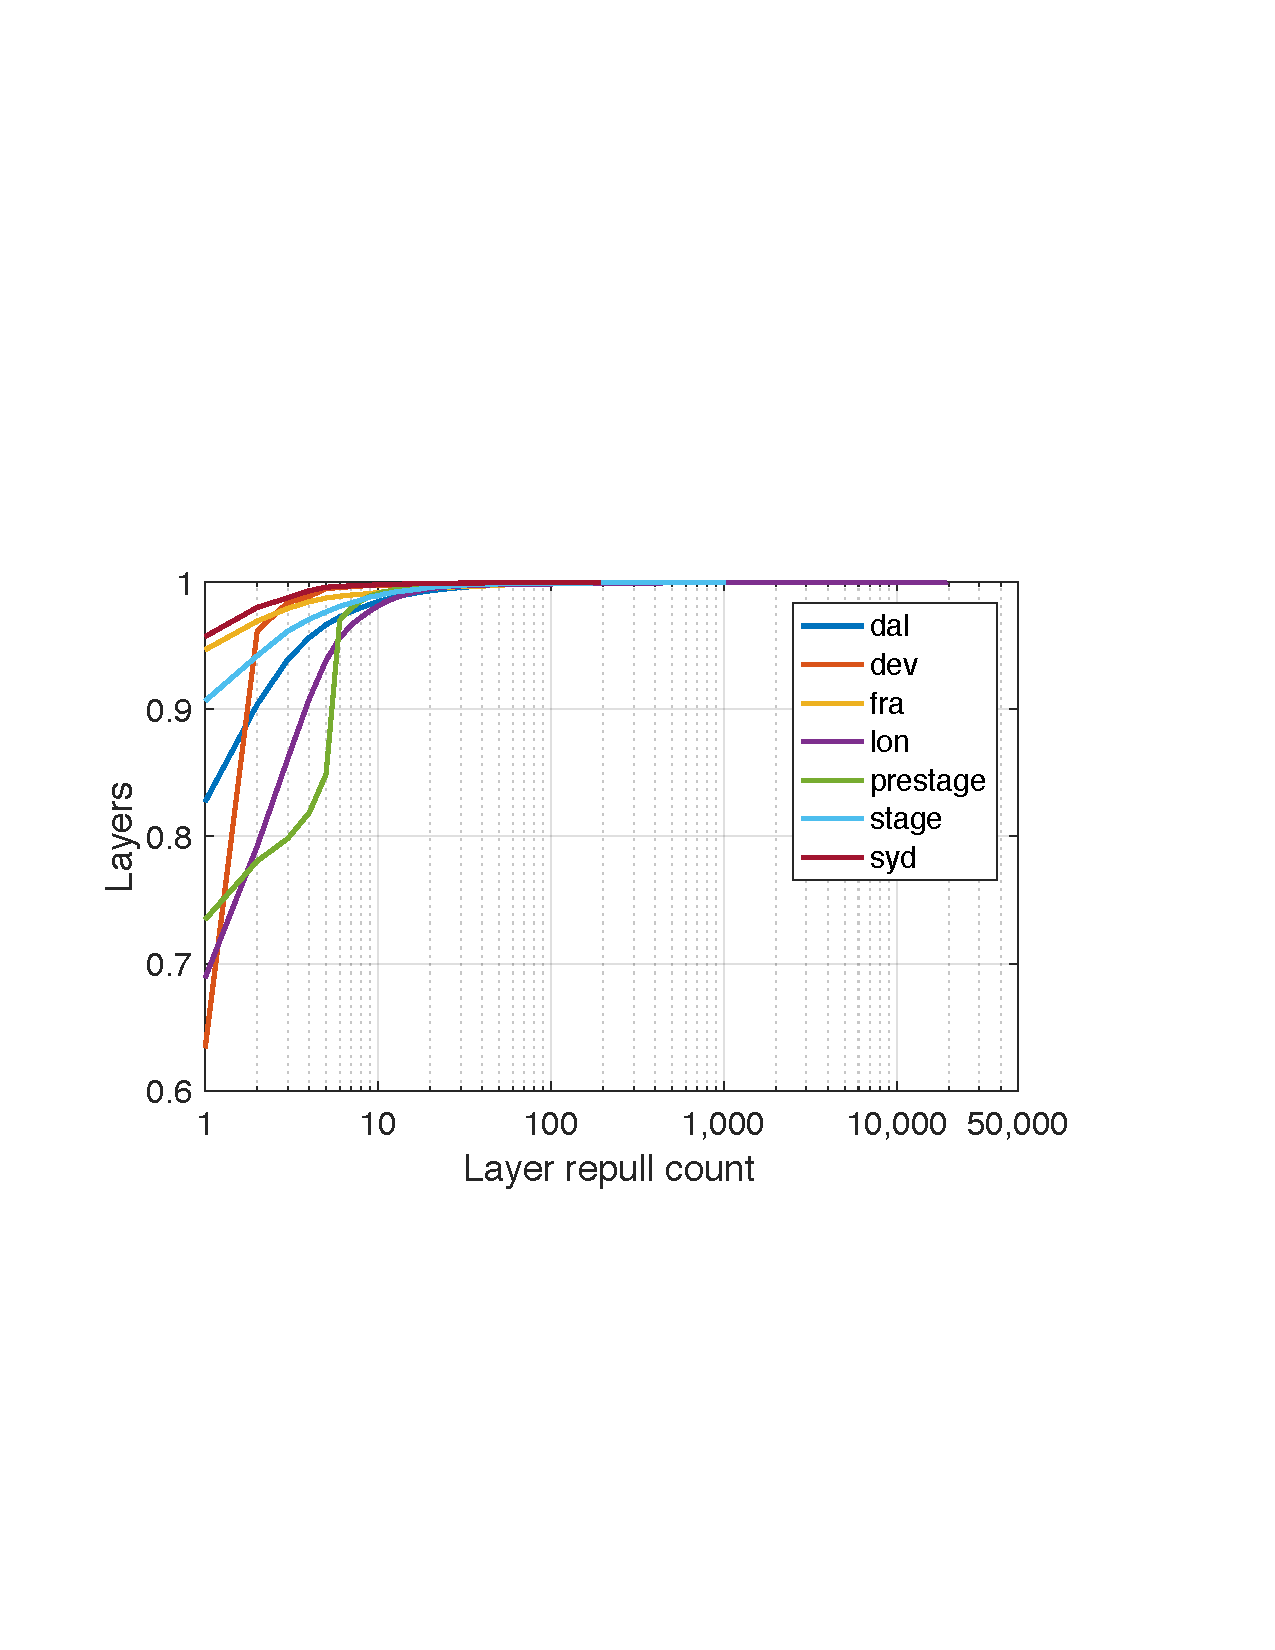
\includegraphics[width=1\textwidth]{graphs/cdf-layer-repull-by-same-client.pdf}
%			%\caption{CDF of layer repull count.}
%		%	\vspace{-3pt}
%			\label{fig:layer-repull-cdf}
%		\end{minipage}
%			\begin{minipage}{0.32\linewidth}
%				\centering
%				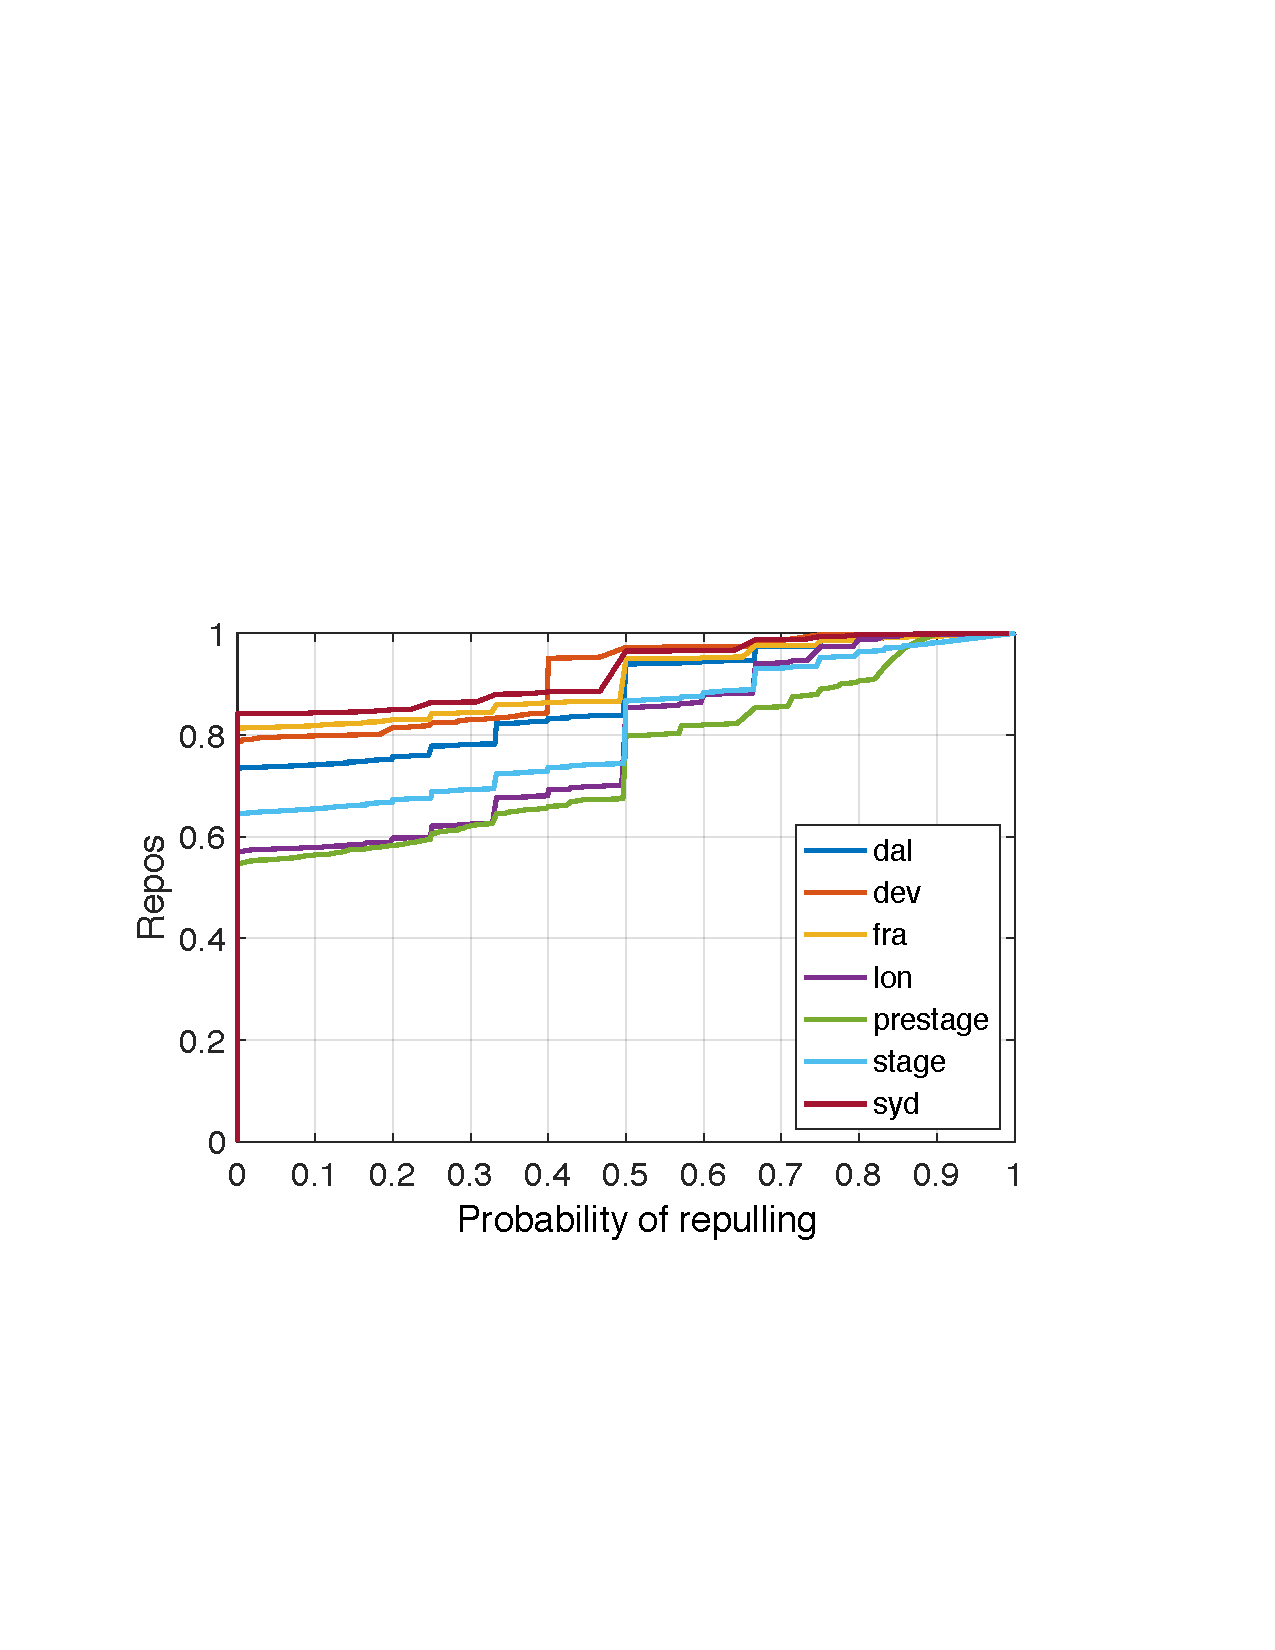
\includegraphics[width=1\textwidth]{graphs/cdf-repo-repull-ratio-by-same-client.pdf}
%				%\caption{PDF of repository repulling probability.}
%				%	\vspace{-3pt}
%				\label{fig:repo-repull-cdf}
%			\end{minipage}
%		\begin{minipage}{0.32\linewidth}
%			\centering
%			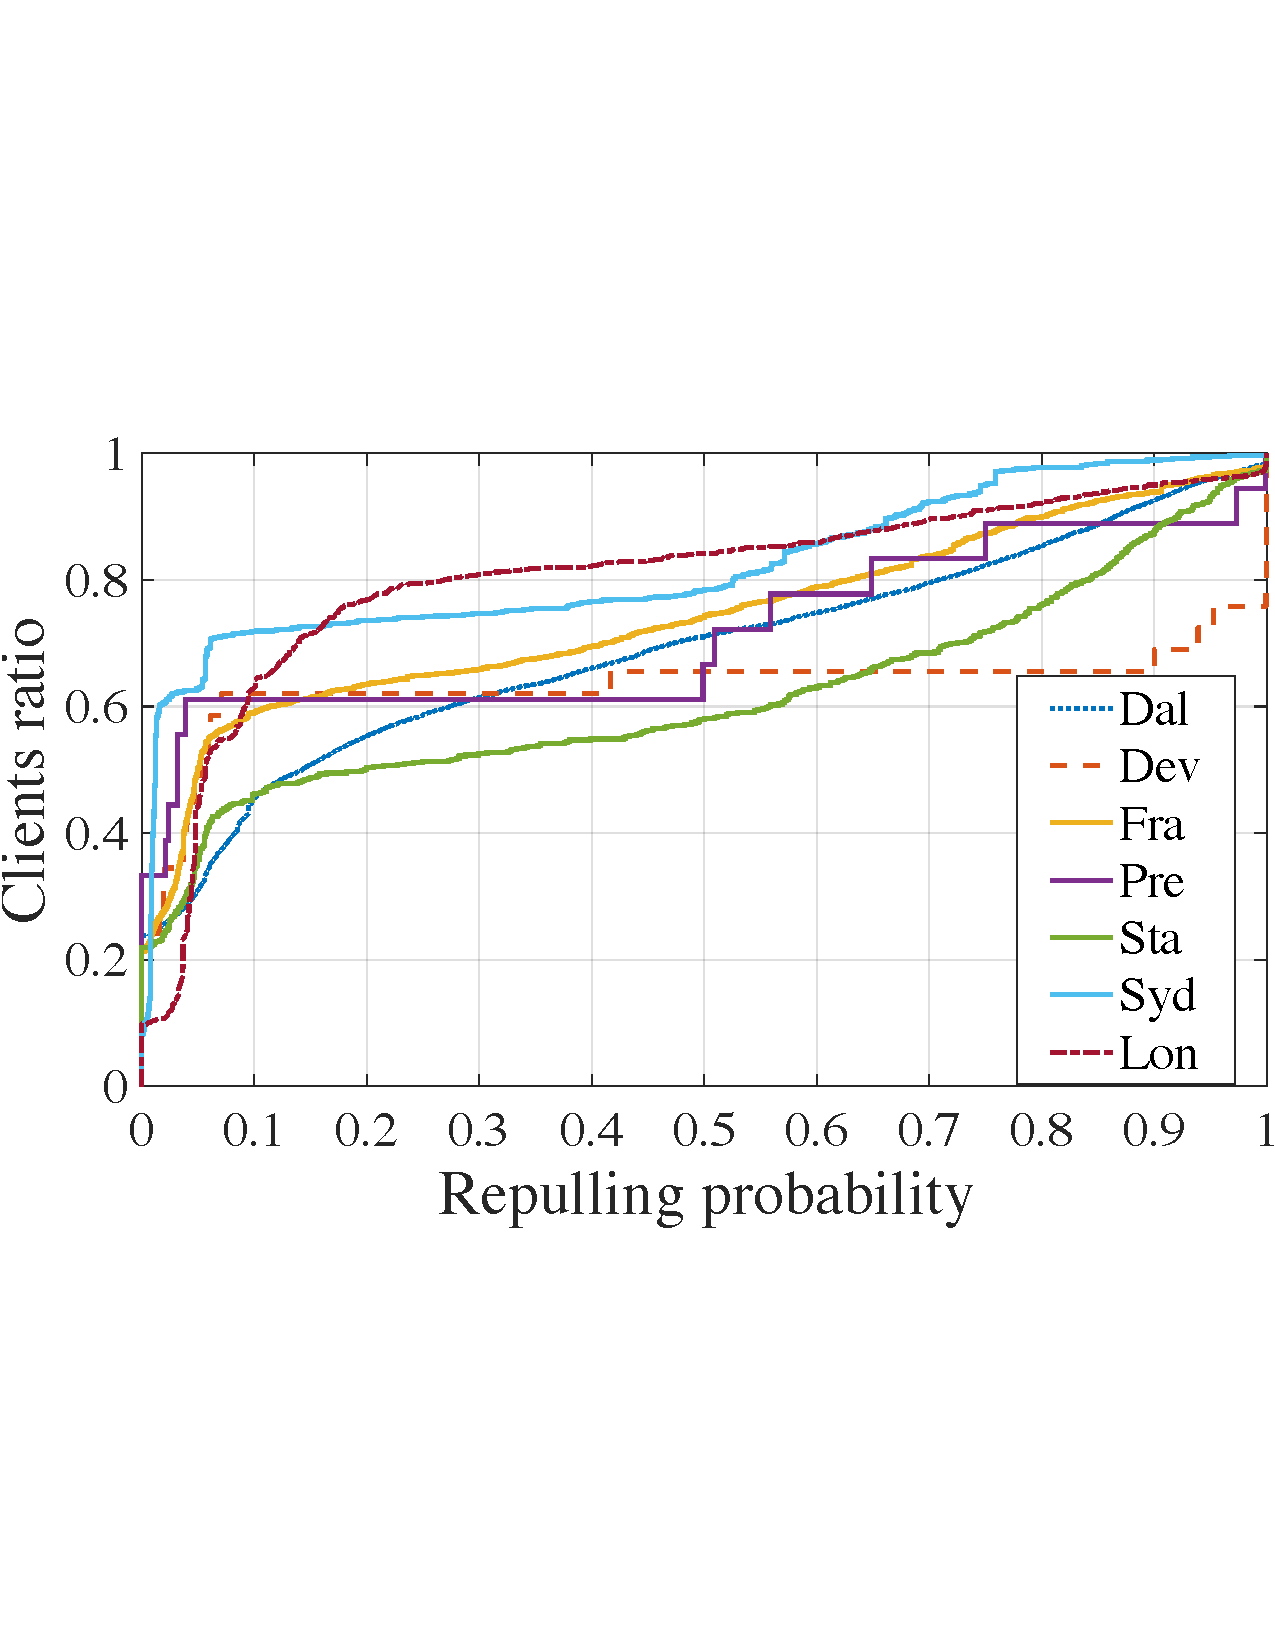
\includegraphics[width=1\textwidth]{graphs/cdf-client-repull-layer-request-ratio.pdf}
%			%
%			%	\vspace{-3pt}
%			\label{fig:client-repull-cdf}
%		\end{minipage}
%	\caption{PDF of client repull count, repository repulling probability, and client repulling probability..}
%\end{figure*}

%\begin{figure}[!t]
%	\centering
%	\subfigure[\texttt{GET} layer request count]{
%		\includegraphics[width=0.22\textwidth]{graphs/cdf-layer-repull-ratio-by-same-client.pdf}
%		\label{fig:layer-repull-cdf}
%	}
%%	\subfigure[Repository repulling probability]{
%%		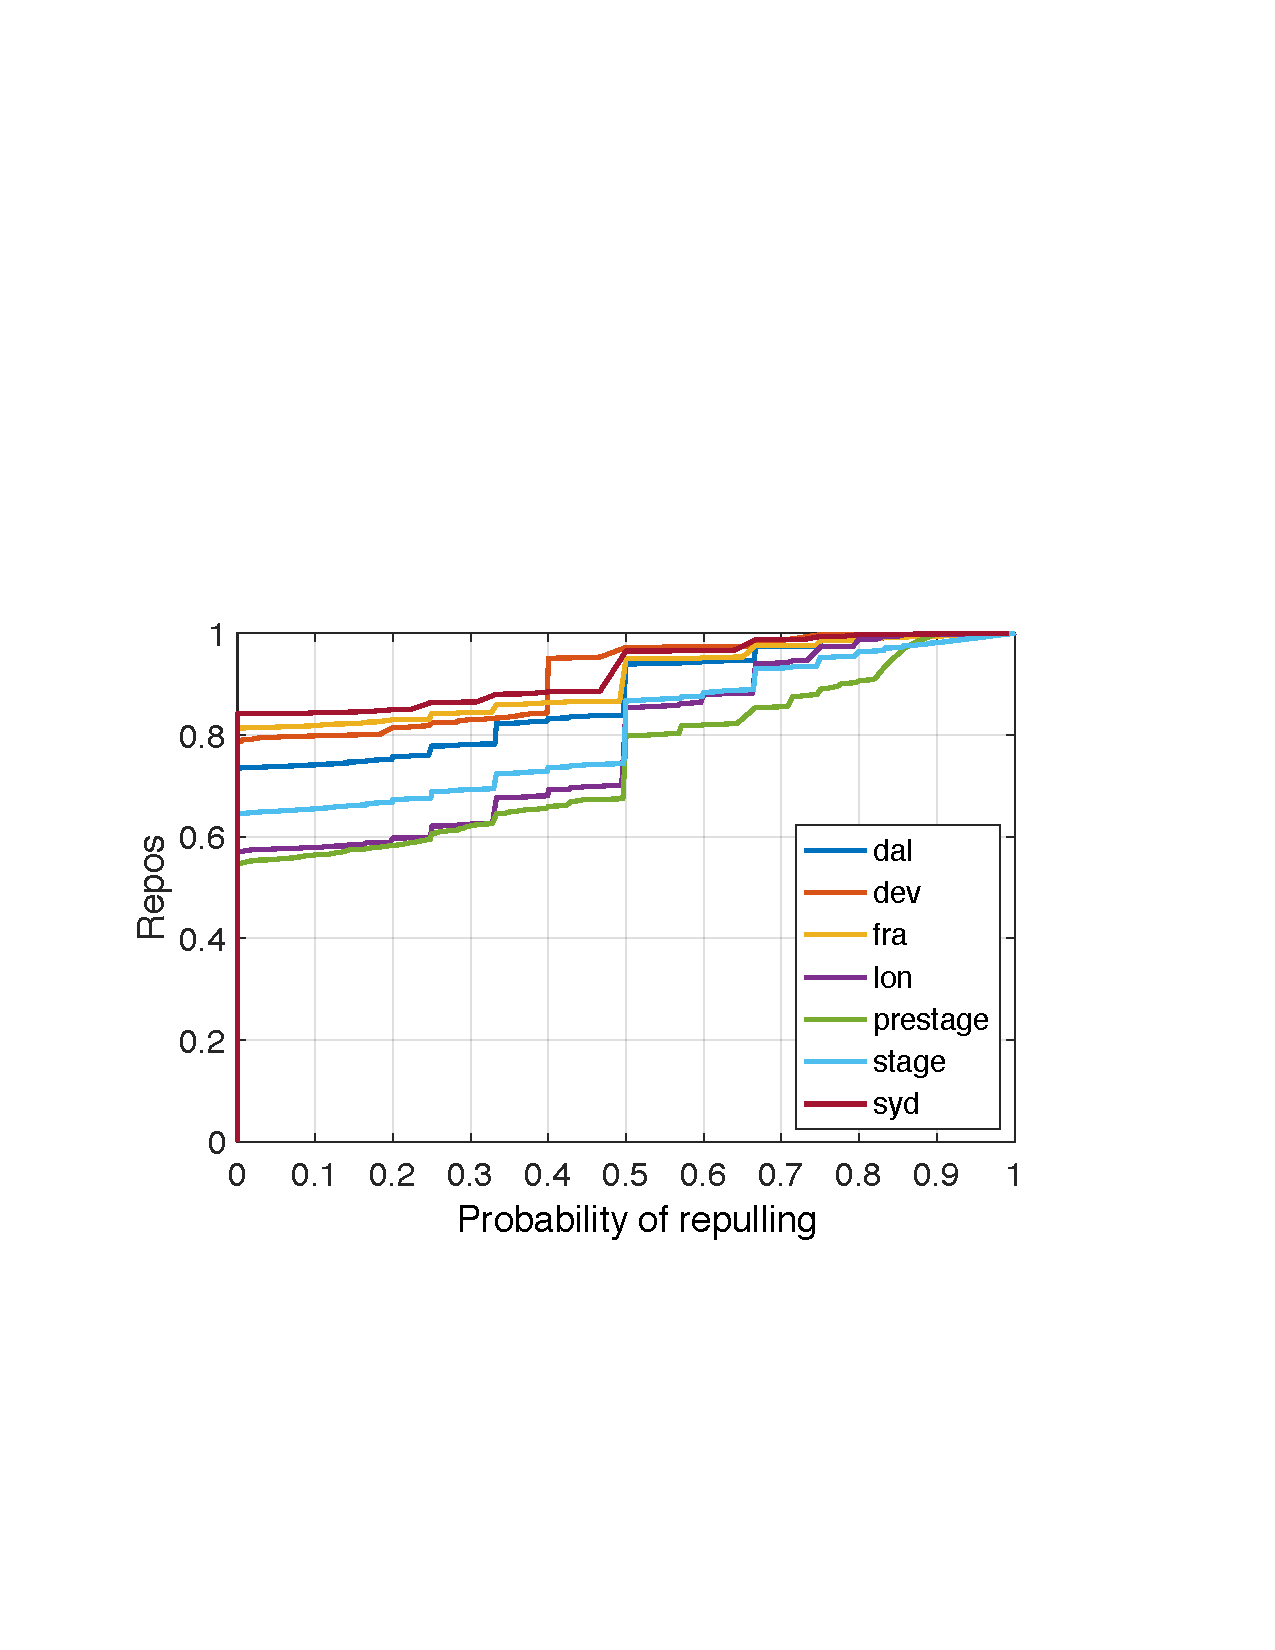
\includegraphics[width=0.2\linewidth]{graphs/cdf-repo-repull-ratio-by-same-client.pdf}
%%		\label{fig:repo-repull-cdf}
%%	}
%	\subfigure[Client repulling probability]{
%	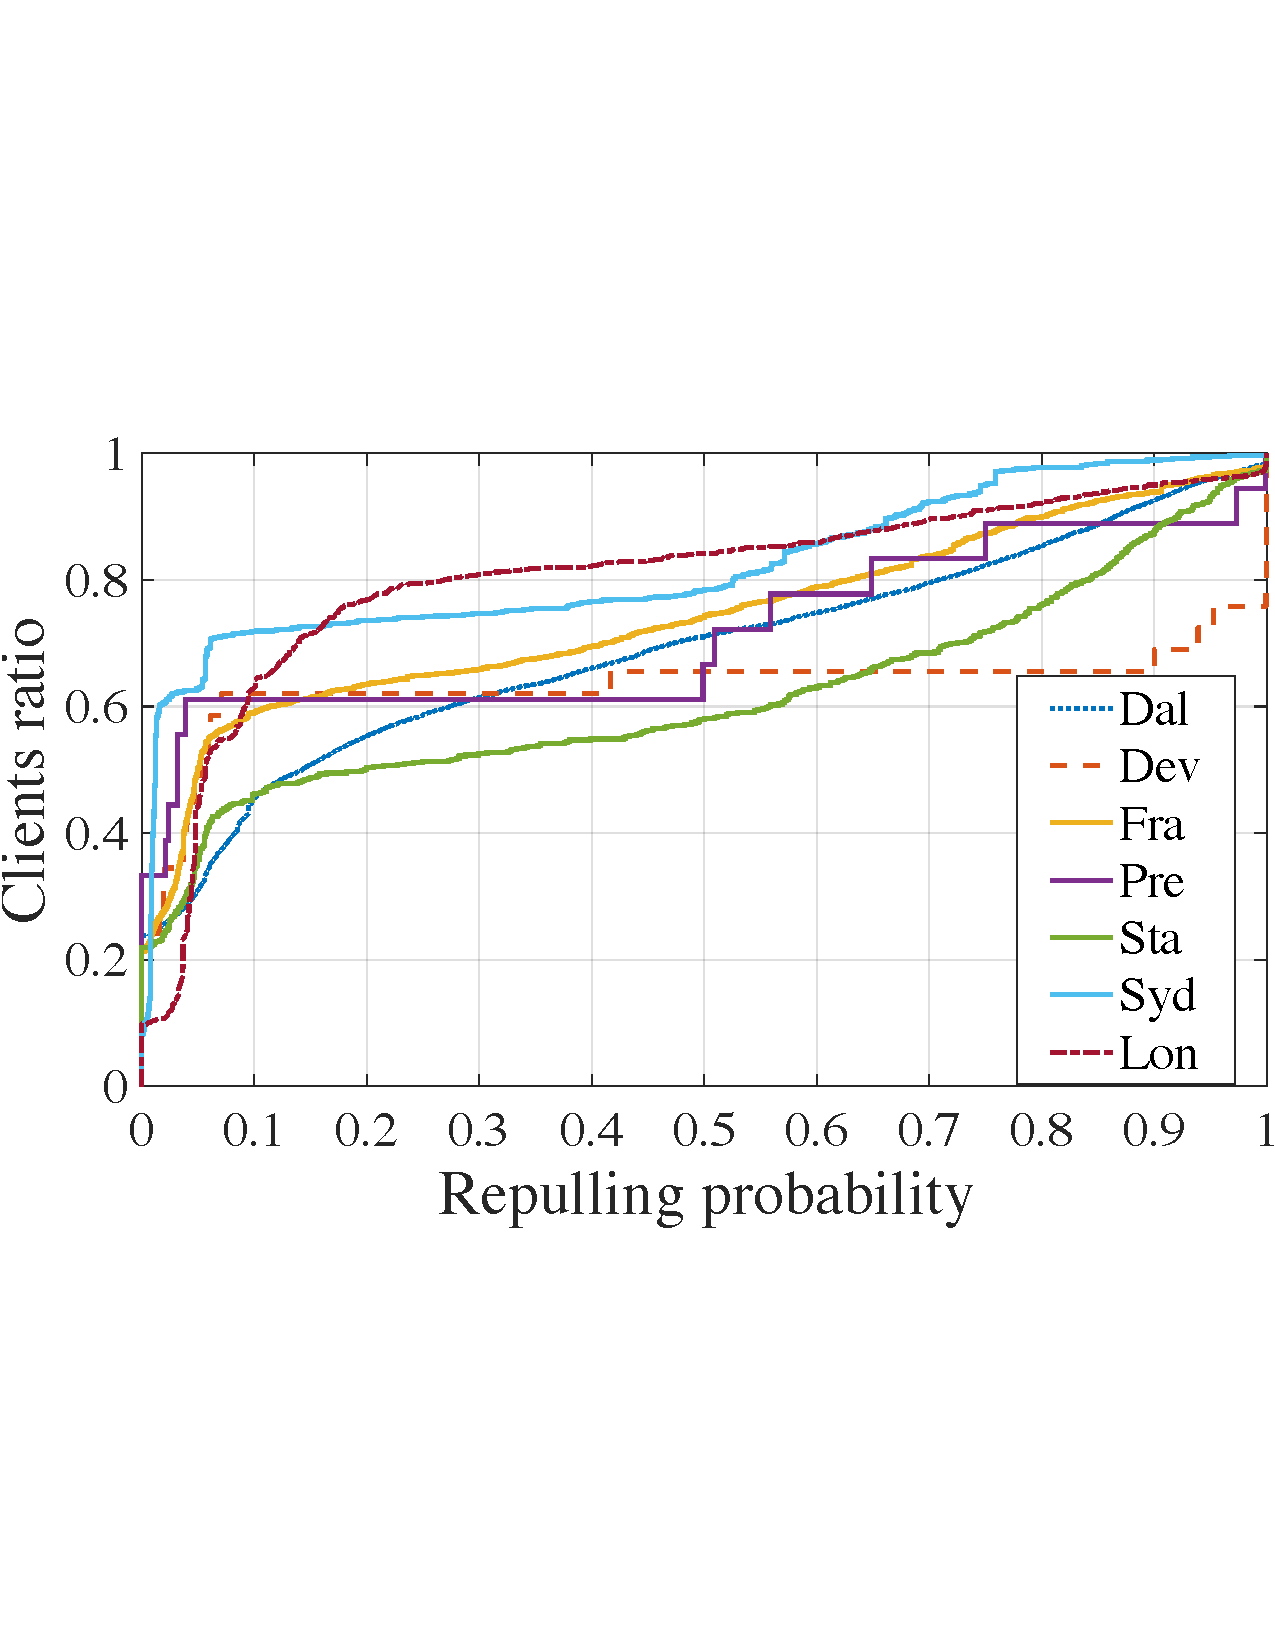
\includegraphics[width=0.2\textwidth]{graphs/cdf-client-repull-layer-request-ratio.pdf}
%   \label{fig:client-repull-cdf}
%}
%	\caption{CDF of \texttt{GET} layer request count and client repulling probability.}
%	\label{fig-repull}
%\end{figure}
%






\begin{figure*}[t]
        \centering
        \begin{minipage}{0.3\textwidth}
                \centering
                \includegraphics[width=0.9\textwidth]{{graphs/cdf-layer-repull-ratio-by-same-client.pdf}
                \caption{CDF of \texttt{GET} layer request count}
                \label{fig:layer-repull-cdf}
        \end{minipage}%
        \begin{minipage}{0.3\textwidth}
                \centering
                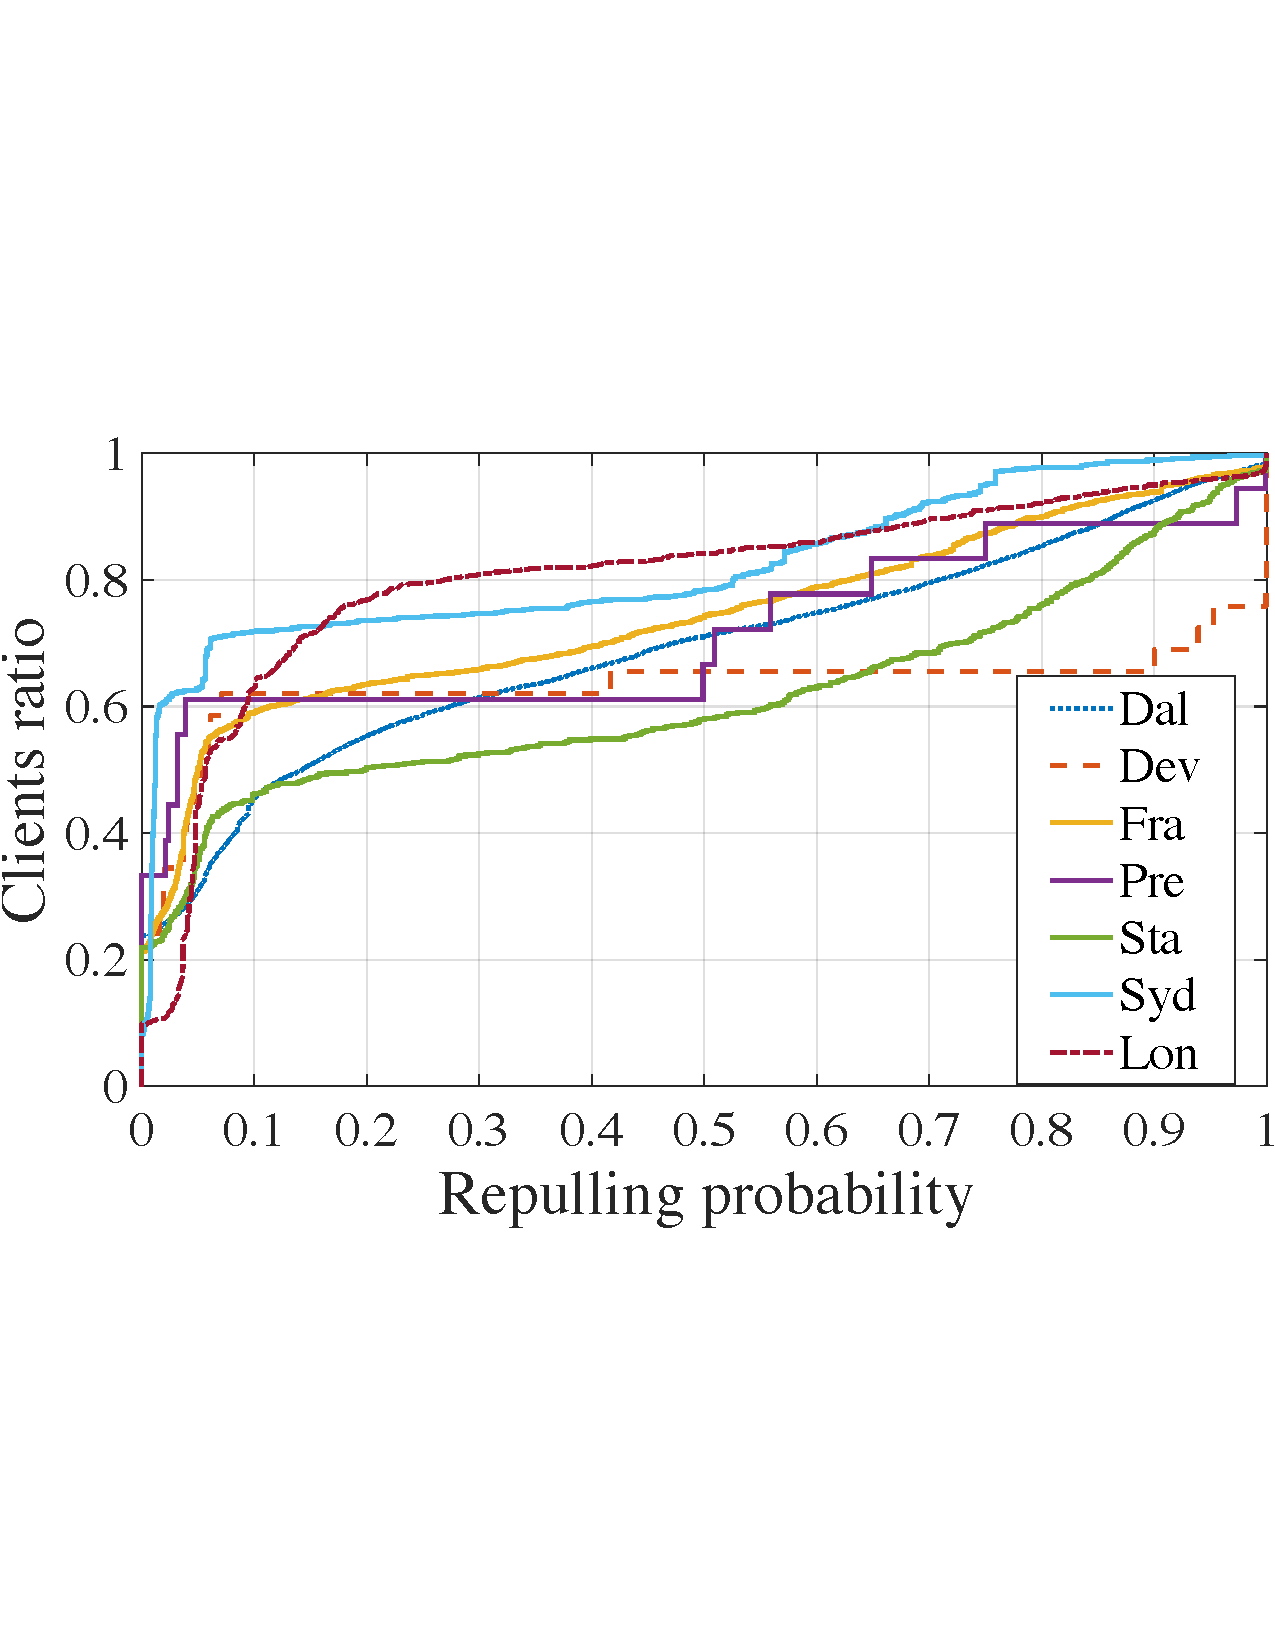
\includegraphics[width=0.9\textwidth]{graphs/cdf-client-repull-layer-request-ratio.pdf}
                \caption{CDF of Client repulling probability}% of LRU cache and preconstruct cache.}
                \label{fig:client-repull-cdf}
        \end{minipage}%
        \begin{minipage}{0.3\textwidth}
        \centering
        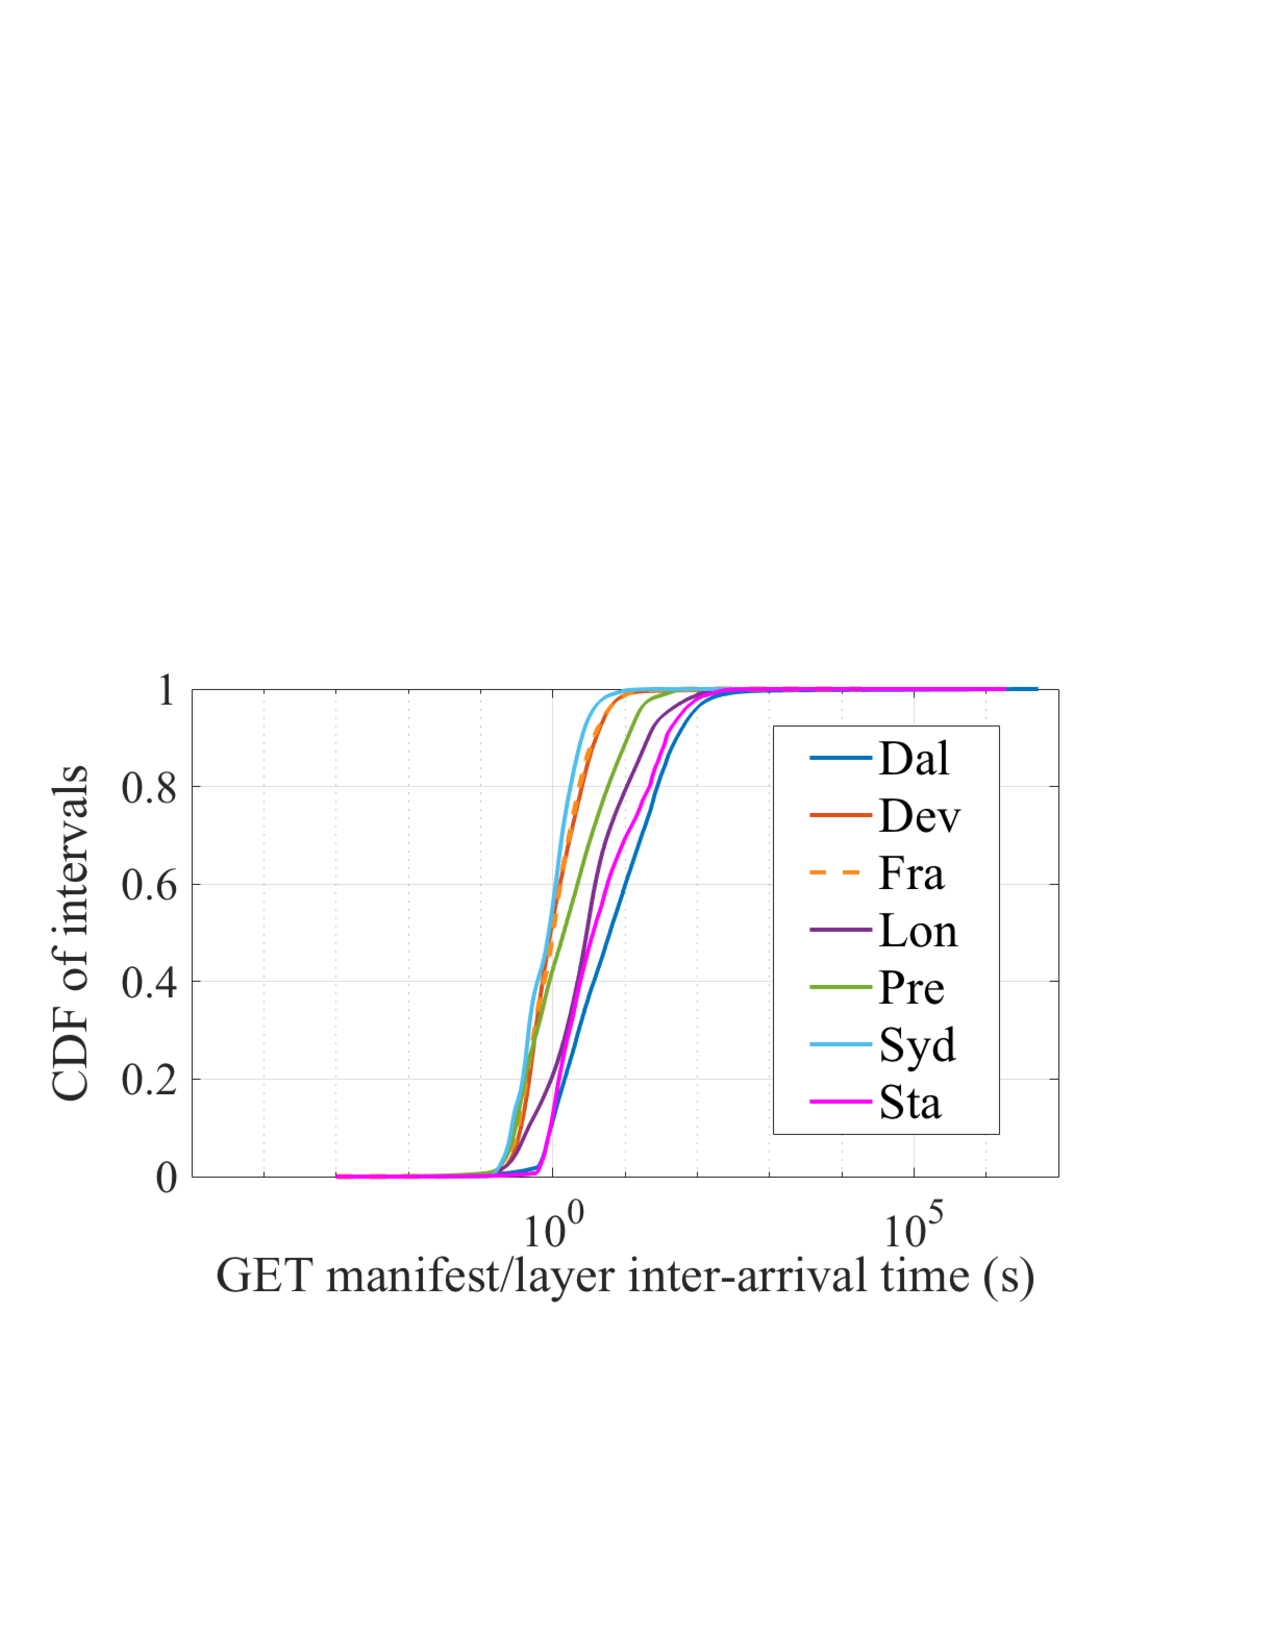
\includegraphics[width=0.9\textwidth]{graphs/GML-intervals.pdf}
        \caption{Intervals between \texttt{GET} manifest request and \texttt{GET} layer request}
        \label{fig:intervals}
   \end{minipage}
\end{figure*}





%\begin{figure}[!t]
%	\centering
%	\subfigure[CDF of compression ratio]{\label{fig_cdf_compression_ratio}
%		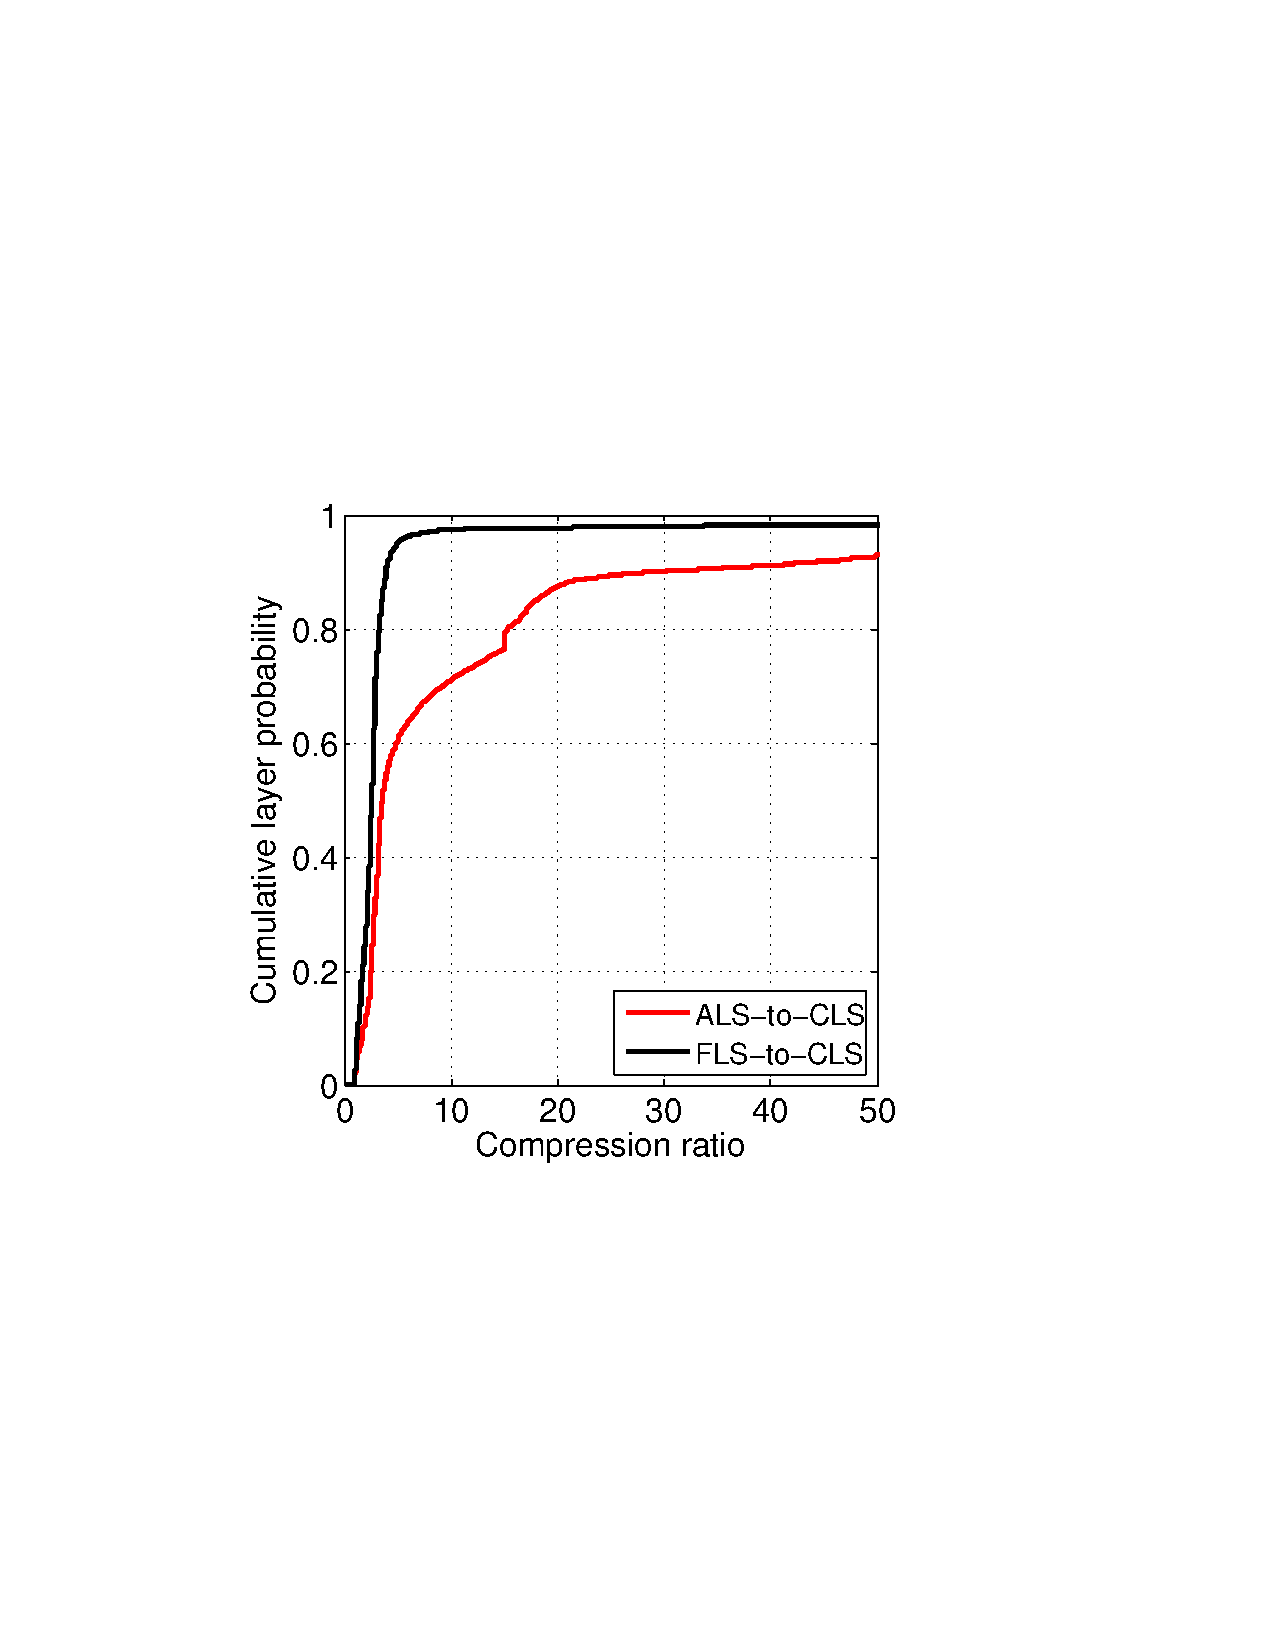
\includegraphics[width=0.23\textwidth]{graphs/cdf_compression_ratio.pdf}
%	}
%	\subfigure[Histogram of comp. ratios]{\label{fig_his_compression_ratio}
%		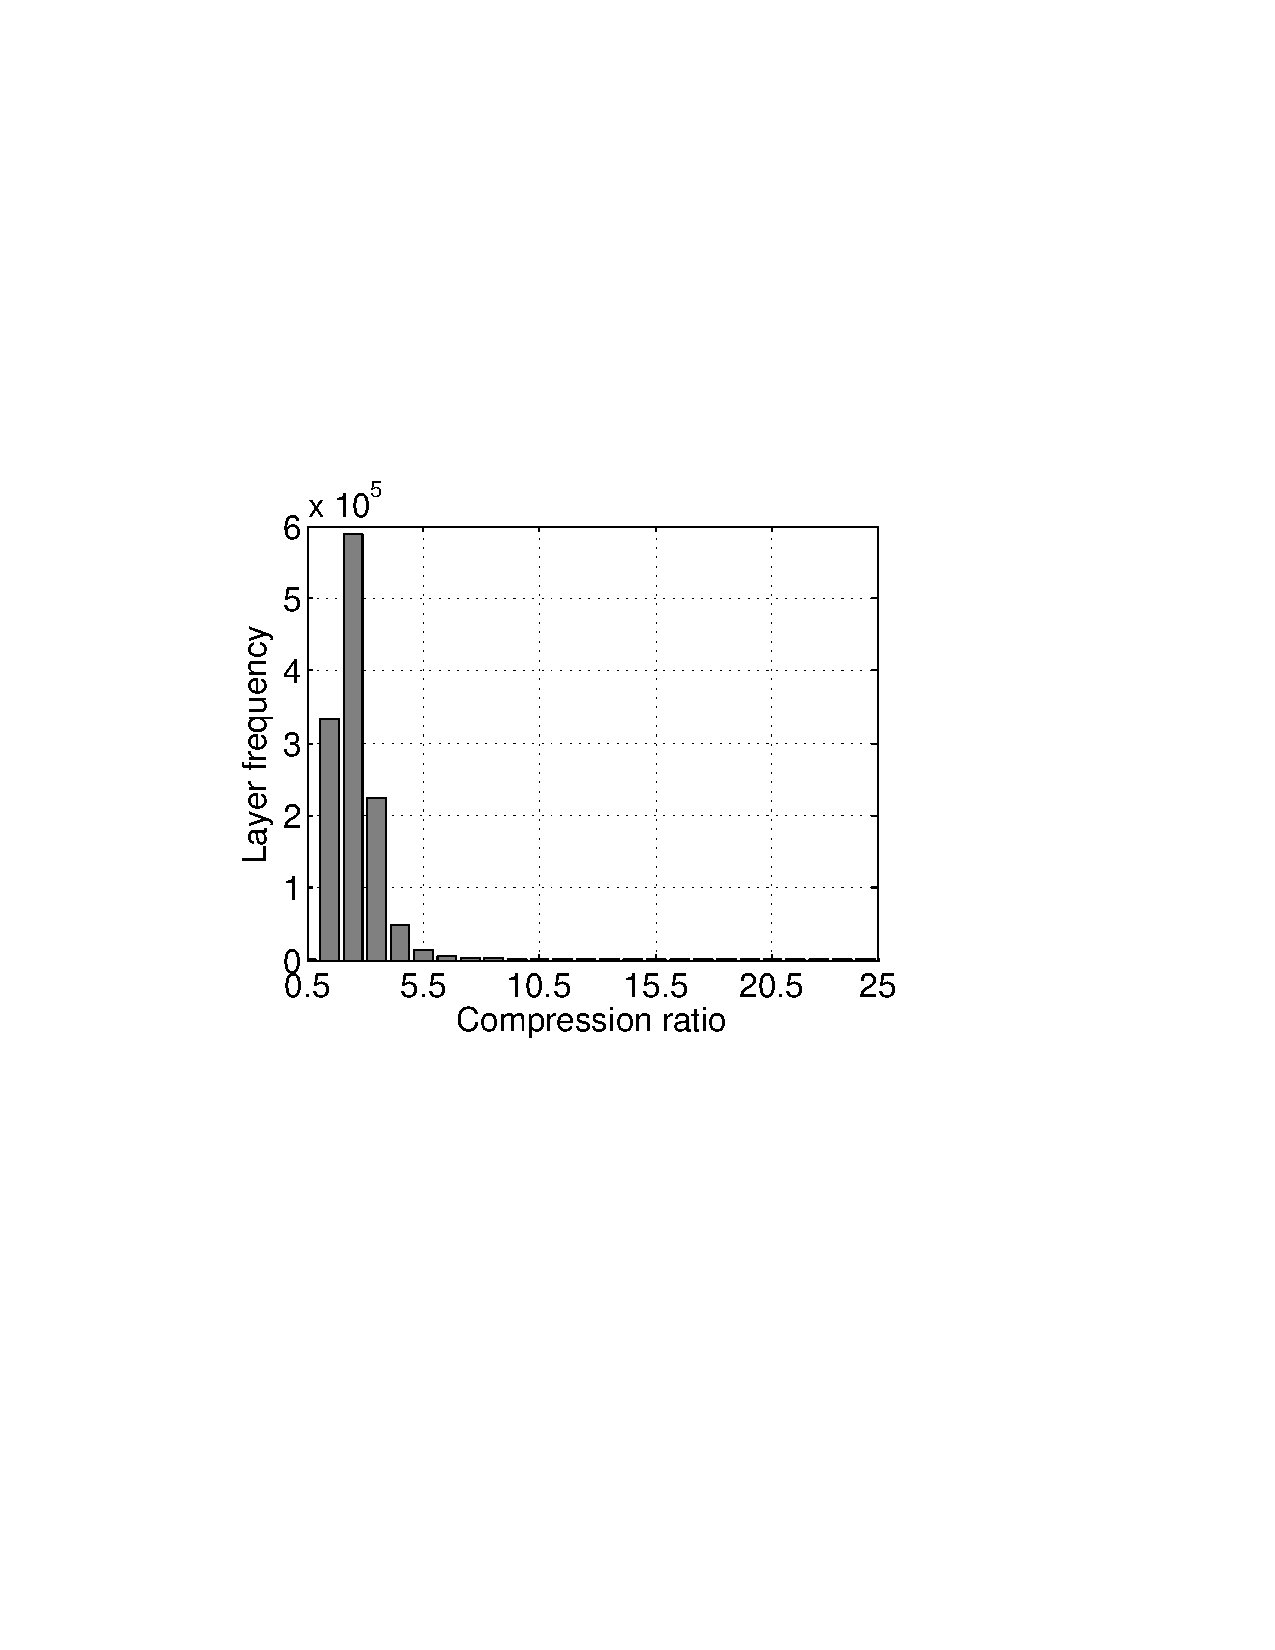
\includegraphics[width=0.223\textwidth]{graphs/his_compression_ratio.pdf}
%	}
%	\caption{Layer compression ratio distribution
%		%\vcomment{Different colors are used in figure (a) and (b) FLS/CLS\nancomment{will address later}}
%	}
%	\label{fig-compression-ratio}
%\end{figure}


%\begin{figure}[t]
%	\centering
%	\begin{minipage}{0.26\textwidth}
%		\centering
%		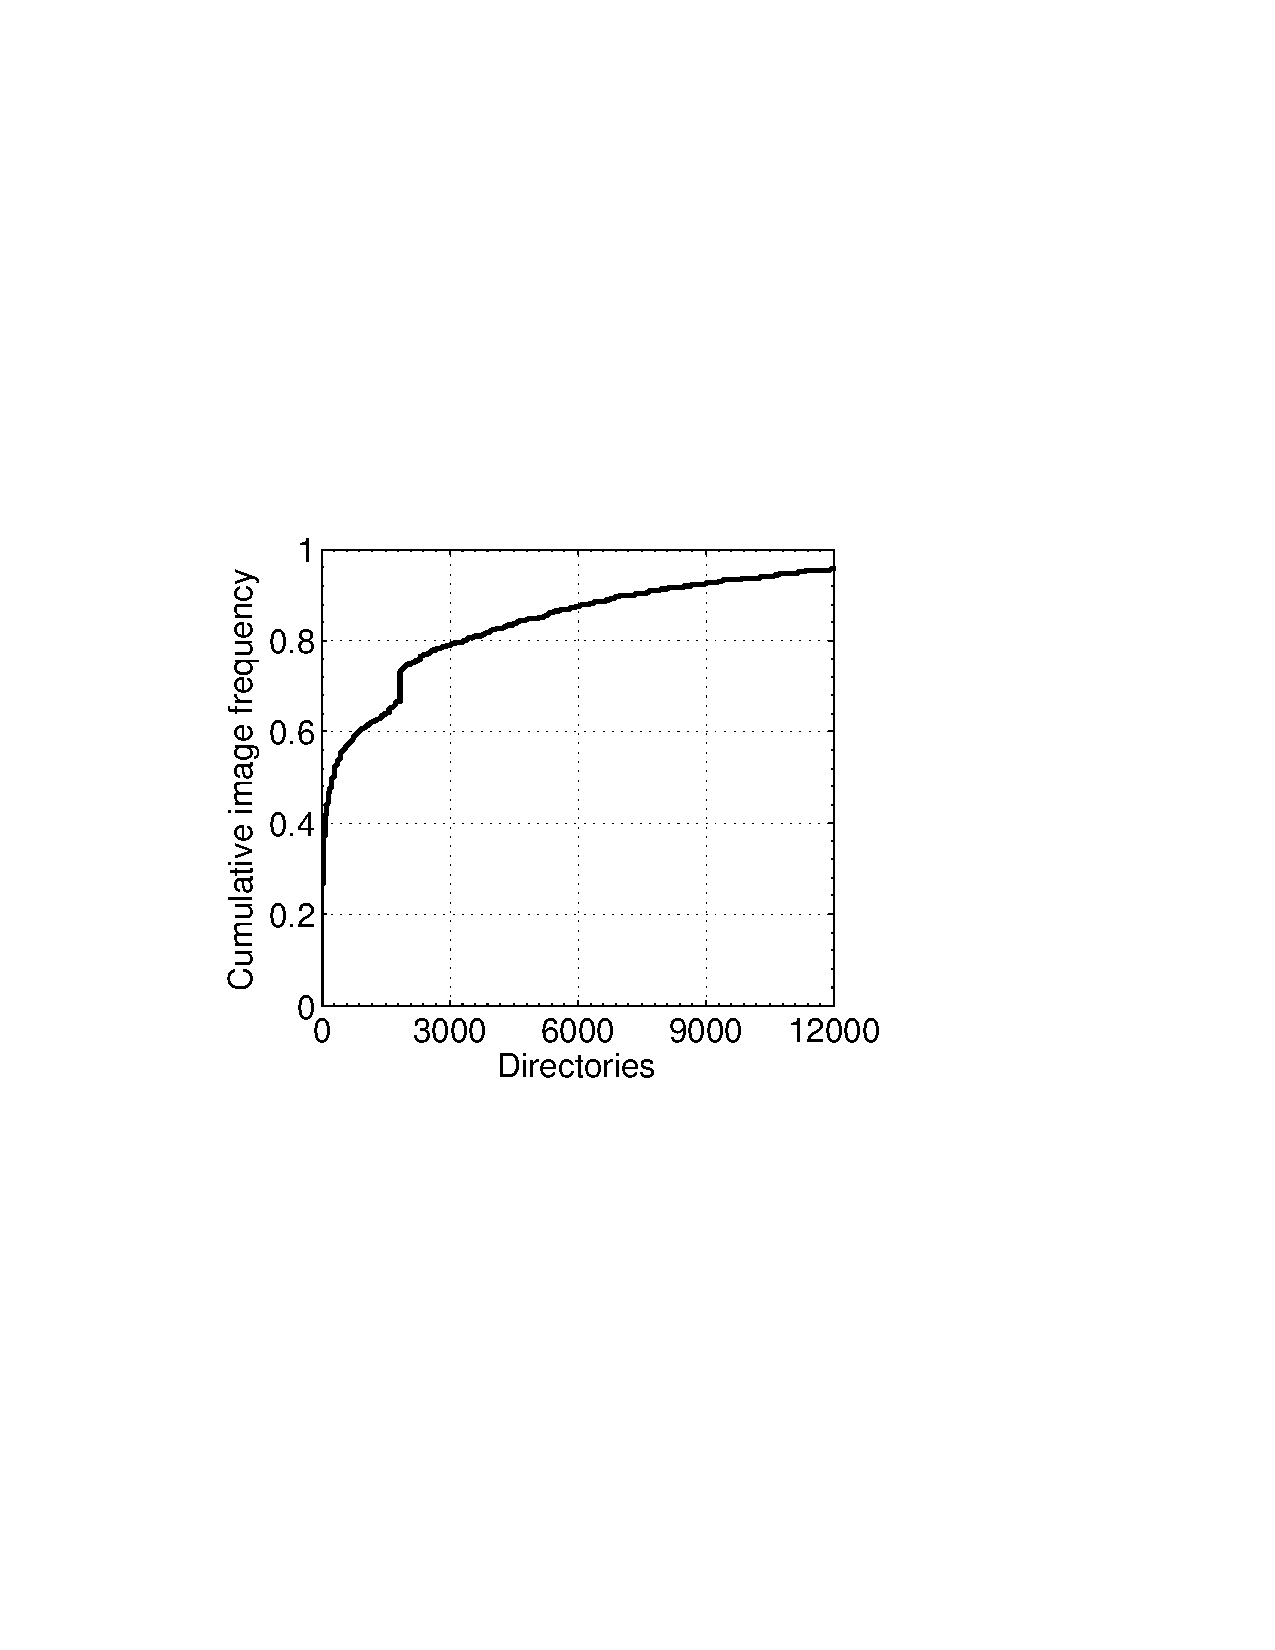
\includegraphics[width=1\textwidth]{graphs/dir.pdf}
%		\caption{CDF of images by\newline directories}
%		\label{fig-dir}
%	\end{minipage}%
%	\begin{minipage}{0.24\textwidth}
%		\centering
%		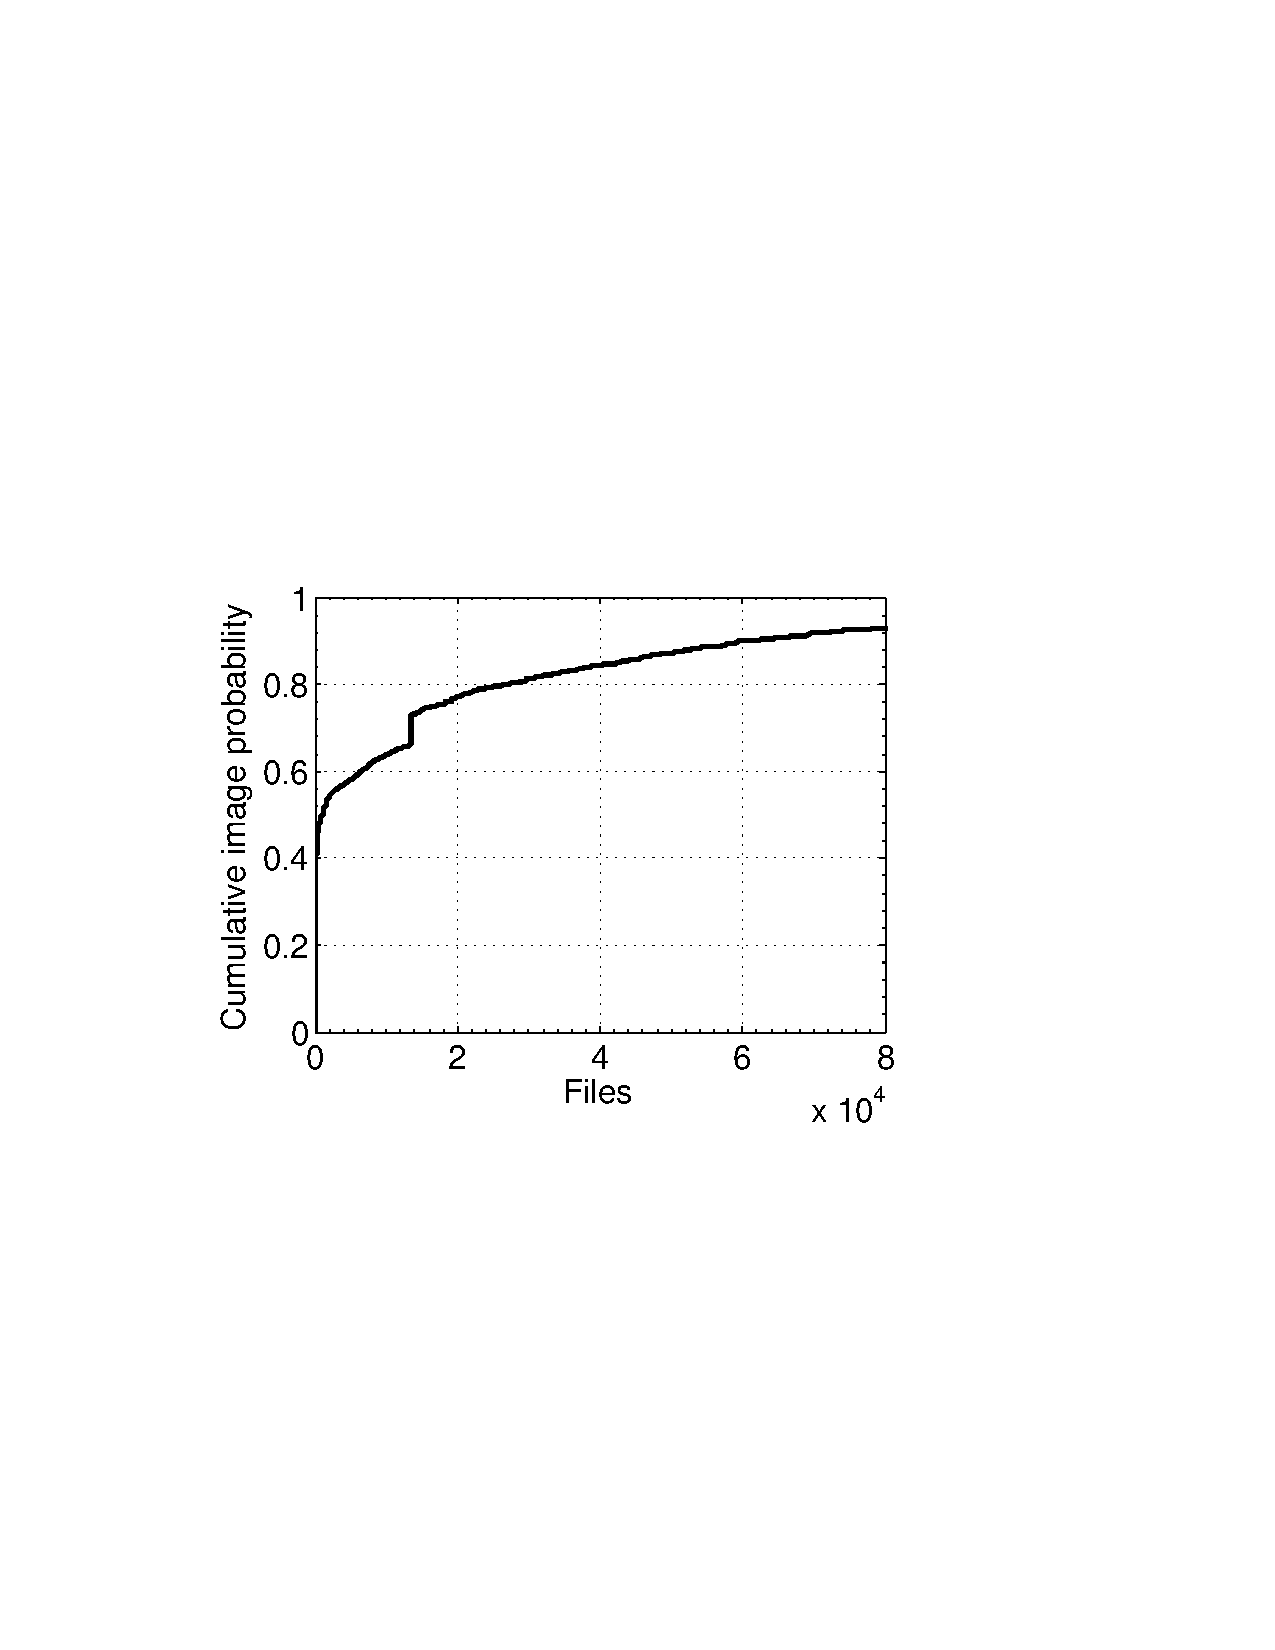
\includegraphics[width=1\textwidth]{graphs/file.pdf}
%		\caption{CDF of images by files}
%		\label{fig-file}
%	\end{minipage}
%\end{figure}

%\begin{figure}[htbp] 
%	\begin{minipage}{0.5\linewidth} 
%		\centering 
%		\includegraphics{circle} 
%		\caption{A Circle} 
%		\label{fig:circle} 
%	\end{minipage}% 
%	\begin{minipage}{0.5\linewidth} 
%		\centering 
%		\includegraphics{rectangle} 
%		\caption{A Rectangle} 
%		\label{fig:rectangle} 
%	\end{minipage} 
%\end{figure}






